\chapter{水库模式}
%\addcontentsline{toc}{chapter}{陆地表面的水分循环}

    本模块在CaMa-Flood中实施水库运行方案,通过识别坝体所在的集水区单元,
    根据水库运行规则计算水库流出量,构建考虑大坝影响的河道汇流参数化方案,
    以刻画水库对陆面水文循环过程的影响。
    
\section{水库数据集和水库参数估计}\label{水库数据集和水库参数估计}
大坝水库的基本信息来自全球大坝水库数据集 GRanD \citep{lehner2011high},GRanD version 1.3 包含全球 7320 座大坝及其相关水库的数据。
本模块需使用数据库中的大坝名称、坝体坐标、总库容和流域面积等信息,然后在 CaMa-Flood 河网上定位水库,并估算水库特征参数。
水库的定位程序包括以下几个步骤:首先根据水库的地理参考坐标计算相应的网格坐标,然后使用河网数据对水库位置进行了校正,
具体来说,将初始水库网格的集水面积与实际值进行比较,如果相对误差大于 10\%,
则对网格的位置进行调整,在周围八个网格进行搜索将流域面积误差降至最低,以此类推直到误差小于10\%。
此外,如果多个水库位于河网中的单个网格中,则模型只选择总蓄水量最大的水库而删除其他水库。通过上述步骤,
在 0.25\textdegree 河网中共计识别到 2169 座水库,在 0.05\textdegree 河网中共计识别到 5715 座水库(图~\ref{fig:水库分布})。

{
\begin{figure}[]
\centering
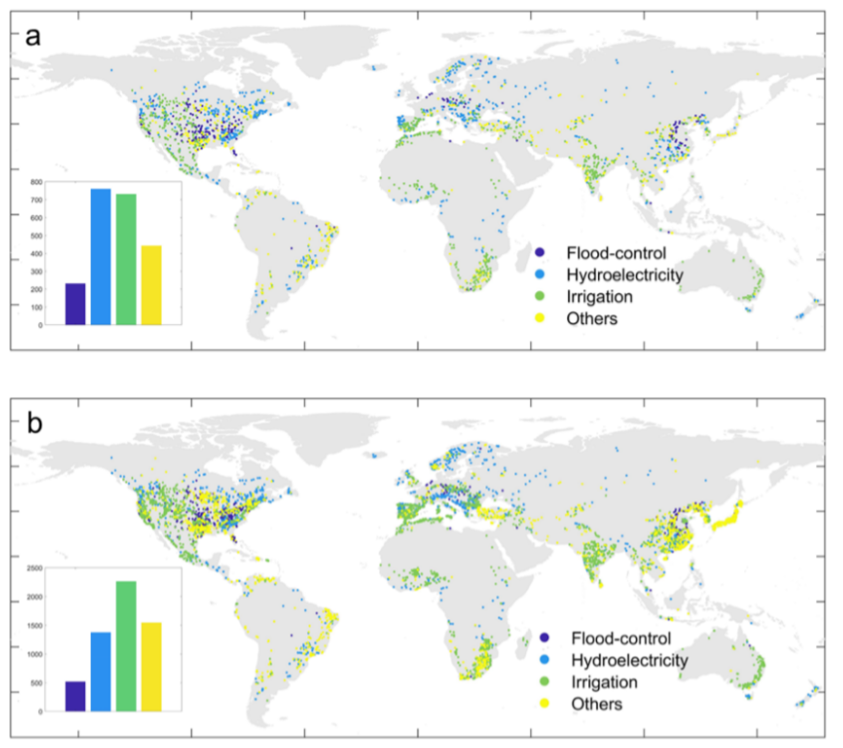
\includegraphics{Figures/陆地表面的水分循环/水库分布.png}
\caption{全球15$'$ (a)和3$'$ (b)河网分辨率下的水库分布。}
\label{fig:水库分布}
\end{figure}
}

水库调度规则参数化方案中所需的水库特征参数包括特征库容 (总库容$V_t$,警戒库容$V_e$、防洪库容$V_f$、
正常库容$V_c$)和特征流量 (防洪流量$Q_f$、正常流量$Q_c$)。
其中,总库容由 GRanD 数据集提供,其他特征库容的提估计需要使用GRSAD~\citep{zhao2019towards}和全球水库形状数据集ReGeo~\citep{yigzaw2018new} 。
GRSAD提供了GRanD中6817个水库1984年至2015年每月水库面积观测数据的时间序列。
ReGeom提供了GRanD中6824个水库的最佳概化几何形状和对应的蓄水\~面积关系数据。
对于防洪库容$V_f$,定义水库水面达最大面积的75\%时(基于GRSAD数据)水库达到了防洪水位和防洪库容,
将此处的面积对照水库形状数据(基于ReGeom数据)即可得到防洪库容。警戒库容$V_e$和正常库容$V_c$则根据以下公式计算:
\begin{equation}
V_{e}=V_{f}+0.8 \times\left(V_{t}-V_{f}\right)
\end{equation}
\begin{equation}
V_{c}=V_{f} / 2
\end{equation}


如图~\ref{fig:水库特征库容示意图} 所示,水库的特征流量包括防洪流量和正常流量,
防洪流量设定为水库设计洪水流量的50\%,正常流量则设定为坝址处的多年平均日径流量。
坝址处的河道流量数据则是基于CaMa-Flood在自然情景下模拟所得。假设水库设计洪水标准为百年一遇洪水,
基于坝址处模拟的3小时径流量数据,采用Gumbel分布估算重现期为100年的设计洪水\citep{boulange2021}。

{
\begin{figure}[]
\centering
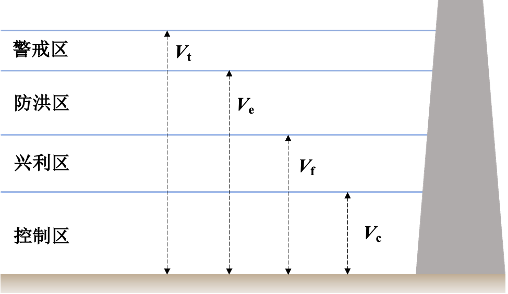
\includegraphics{Figures/陆地表面的水分循环/水库特征库容示意图.png}
\caption{水库特征库容示意图。}
\label{fig:水库特征库容示意图}
\end{figure}
}
\section{水库调度规则参数化方案}
在大尺度陆面模式中进行水库扰动模拟,需要对水库的调度规则进行一定的假设和概化,现有方案大致可分为三类:
基于入流和需求的调度方案、基于离线优化的调度方案和基于目标库容的分段调度方案,
其中基于目标库容的方案在高性能 (计算的简单性和透明性) 与全球适用性 (适用场景的代表性和广泛性) 之间能够取得较好的平衡\citep{yassin2019representation}。
因此,本模块的水库调度方案采用基于目标库容的分段调度方式,将水库库容分为四个特征库容区 (如图~\ref{fig:水库特征库容示意图}所示),
不同用途的水库主要区别就在于兴利区和防洪区的调度目标和出流规则。本模块包括了以防洪和需水为目标的水库调度参数化方案。


防洪调度方案根据水库入流量、库容大小和库容调节能力,调节出库流量以削减汛期峰值流量,
控制出库流量不超过防洪流量,且根据汛期发展时段调整出流系数 \citep{hanazaki2022development}:\\
警戒区:
\begin{equation}
Q=\max \left(Q_{f}, I\right)
\end{equation}
防洪区:
\begin{equation}
Q=\begin{cases}
Q_{f}+k \frac{V-V_{f}}{V_{e}-V_{f}}\left(I-Q_{f}\right), & \text{当}\quad I \geq Q_{f} \\
Q_{n} \times 0.5+\left(\frac{V-V_{c}}{V_{e}-V_{c}}\right)^{2}\left(Q_{f}-Q_{n}\right), & \text{当}\quad I<Q_{f}
  \end{cases}
\end{equation}
兴利区:
\begin{equation}
Q=\begin{cases}
Q_{n} \times 0.5+\left(\frac{V-V_{c}}{V_{f}-V_{c}}\right)\left(Q_{f}-Q_{n}\right), & \text{当}\quad I \geq Q_{f} \\
Q_{n} \times 0.5+\left(\frac{V-V_{c}}{V_{e}-V_{c}}\right)^{2}\left(Q_{f}-Q_{n}\right), & \text{当}\quad I<Q_{f}
  \end{cases}
\end{equation}
控制区:
\begin{equation}
Q=Q_{n} \times\left(\frac{V}{V_{f}}\right)
\end{equation}
其中:$I$表示入库流量,$Q$表示出库流量,$V$表示实际库容,$V_e$表示警戒库容,
$V_f$表示防洪库容,$V_c$表示正常库容,$Q_f$表示防洪流量,$Q_n$表示正常流量,$k$表示出流调节系数,
取值为$\max(1-(V_t-V_f)/A,0)$,$A$为水库上游面积,$V_t$为水库总库容。特征库容和特征流量的提取如章节~\ref{水库数据集和水库参数估计} 所述。


需水调度方案则根据水库下游需水量、入库流量、实时库容大小调节出流,以满足水库服务区域内的用水需求 \citep{hanasaki2006reservoir,shin2019high}:\\
警戒区:
\begin{equation}
Q=\max \left(Q_{f}, I\right)
\end{equation}
防洪/兴利区:
\begin{equation}
Q=\begin{cases}
  (1-R) I+R \times \frac{V-V_{c}}{V_{f}-V_{c}} \times\left(Q_{n}+D-\bar{D}\right) & \text{当}\quad
    \bar{D} / Q_{n}<1-M \\ 
  (1-R) I+R \times \frac{V-V_{c}}{V_{f}-V_{c}} \times Q_{n}\left(M+\frac{(1-M) D}{\bar{D}}\right)      &  \text{当}\quad \bar{D} / Q_{n}>M
    \end{cases}
\end{equation}
控制区:
\begin{equation}
Q=Q_{n} \times\left(\frac{V}{V_{f}}\right)
\end{equation}
其中:$\bar{D}̅$表示多年平均日需水量,$D$表示当日需水量,
$M$表示最小需求满足系数 (默认取值为0.5 \citep{hanasaki2006reservoir}),$R$表示需求决定系数,
取值为$\min \left(1, \alpha\left(\frac{V_{f}-V_{d}}{Q_{n}}\right)^{2}\right)$,
$\alpha$为经验参数 (默认取值为4 \citep{hanasaki2006reservoir}),其他变量含义同上式。


\section{考虑大坝影响的河道汇流参数化方案}
当水库网格处的蓄水量和水位在水库运行期间增加时,考虑回水影响的模型 (例如CaMa-Flood) 中可能会出现上游回水 (storage buffering effect),
洪水期间河流蓄水量的增加受到水库上游回水的缓冲,将使得模拟入流量波动较小。因此,相比自然河道的汇流方案,考虑大坝影响的汇流方案存在以下改动:
当河道中存在大坝时,由于水的连续流动和河道的水力连结被切断,在与大坝网格紧连的下游网格处,圣维南动力方程中的局部加速项和静水压力项被忽略,
在使用局部惯性方程 (CaMa-Flood中使用的默认算法) 进行一般计算后,使用运动波动方程重新计算流量。
在下一步中,将来自上游河网的所有流出汇总为水库流入,并根据重新计算的流入和蓄水量确定水库流出。
\begin{equation}
g A \frac{\partial z}{\partial x}+\frac{g n^{2}|Q| Q}{R_{H}^{4 / 3} A}=0
\end{equation}
式中变量含义同章节~\ref{诊断洪泛状态} 所述。


此外,由于大坝对汇流过程的拦截作用,在计算大坝网格下游格点的河道蓄水和淹没时,
质量连续方程中的汇流网格和汇流面积将不再包括大坝网格上游的部分,
且与大坝网格紧连的下游网格其入流径流量替换为水库出流量。
\begin{equation}
S_{i}^{t+\Delta t}=S_{i}^{t}+\sum_{k}^{Upstream-2} Q_{k}^{t} \Delta t-Q_{i}^{t} \Delta t+A c_{i} R_{i}^{t} \Delta t
\end{equation}
式中$Upsteam-2$表示在原上游网格的基础上除去大坝上游网格 (例如图~\ref{fig:大坝对下游河道汇流计算方案的影响示意图} 所示),其他变量含义同章节~\ref{诊断洪泛状态} 所述。

{
\begin{figure}[]
\centering
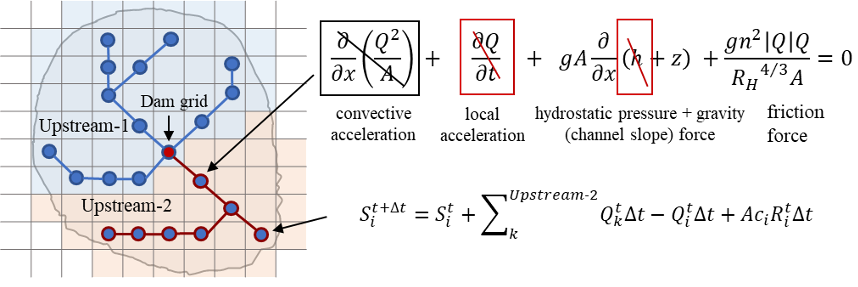
\includegraphics{Figures/陆地表面的水分循环/大坝对下游河道汇流计算方案的影响示意图.png}
\caption{大坝对下游河道汇流计算方案的影响示意图。}
\label{fig:大坝对下游河道汇流计算方案的影响示意图}
\end{figure}
}
